\documentclass[a4paper, 12pt]{article}
\usepackage{amsmath}
%\usepackage[utf16]{inputenc}
\usepackage{graphicx}
\usepackage[left=2.5cm, right=2.5cm, bottom=2.5cm, top=2.5cm]{geometry}
\usepackage{natbib}
\usepackage{microtype}
\usepackage{coloremoji}

\title{Measure --- or as the kids call it these days, addition}
\author{Brendon J. Brewer}
\date{}

\begin{document}
\maketitle

% Need this after the abstract
\setlength{\parindent}{0pt}
\setlength{\parskip}{8pt}

\section{Bigger and smaller}
Some things are bigger than others.

\section{How long is a piece of string?}

Consider a set, or collection, of objects, and suppose we can
unambiguously rank or sort the objects. For example, maybe we
have twenty apples, each of which has been weighed precisely.
We could put the apples in order by mass, from lowest to highest (or
the other way around).

More formally, think of a set $\mathcal{S} = \{s_1, s_2, ..., s_n\}$.
If we can take any two elements
(call them $x$ and $y$) and say that either $x > y$ or $y > x$ (where
we get to define what ``greater than'' means for a particular application),
then $\mathcal{S}$ is a {\em totally ordered set}. The definition of
$>$ that you use has to have the properties that $>$ usually does. For
example, if $x > y$ and $y > z$, then $x > z$. 
Later, there will be a concept called a {\em chain} which is pretty much
the same as a partially ordered set.
If you are used to computer programming, then any
list/vector/array of items which can be unambiguously sorted
is a totally ordered set.

We can draw this situation using points on a line
(Figure~\ref{fig:totally_ordered_set}).
Each point
represents an element of the set, and they are arranged from highest
to lowest in terms of which elements are ``greater than'' other elements.
That is, if $x > y$ (element
$x$ is ranked above element $y$), then $x$ is drawn above $y$ in the
diagram.

\begin{figure}[!ht]
\centering
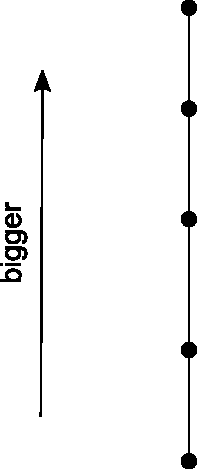
\includegraphics[scale=0.6]{figures/totally_ordered_set.pdf}
\caption{A set with five elements, each represented by a black dot.
When one dot is above another and they are connected with a line, it
means the higher element is greater than (using whatever definition of $>$ we
choose) the lower one.
This is a simple example of a {\em Hasse diagram}. More complex
Hasse diagrams will appear later.\label{fig:totally_ordered_set}}
\end{figure}


\section{The sum rule}

\section{Measure in boolean lattices}


\begin{figure}[!ht]
\centering
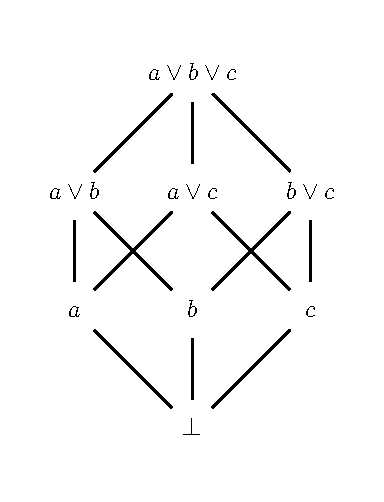
\includegraphics[width=0.5\textwidth]{figures/boolean_lattice.pdf}
\caption{\label{fig:boolean_lattice}}
\end{figure}


Apples.
One bag of apples combined with another bag of apples.
The exact same situation. The numbers of apples add, as
do the masses. Two different sum rules apply to the same
situation!


\section{Infidelity and ``signed measure''}

\subsection{A fate worse than death}

Infidelity allows for fates worse than death.
An absence of experience, denoted $\bot$,
has measure zero, so you can add arbitrary amounts
of non-existence to any experience without changing
its quality. So, for example:
\begin{align}
m(😃 \vee \bot)        &= m(😃)\\
m(😀 \vee 😪 \vee \bot) &= m(😀 \vee 😪)
\end{align}
and so on.
In other words, $\bot$ is the {\em identity element}
of the set of potential experiences.


\end{document}

